\chapter{Sistema hardware}

\bigskip
En esta parte me dedicaré a profundizar en las parte más tangible del proyecto, introduciendo así en la electrónica, 
mecánica y programación a más bajo nivel.

\bigskip
Es importante destacar que gracias a diferentes plataformas de hardware libre he podido reducir en gran parte el alcance del proyecto, pudiendo así centrarme en implementar las funcionalidades y no tanto en montar todo el marco de trabajo 
necesario para llegar a ello. 

\bigskip
Teniendo presentes las  herramientas de última generación, que en la actualidad están teniendo un gran auge y aceptación 
en la comunidad DIY \cite{DIY} "hágalo usted mismo", como lo son las impresoras en 3D o las cortadoras láser, que agilizan la mecanización y fabricación de las partes mecánicas.

\section{Fases}

\begin{itemize}
	\item \textbf{Fase 0:} Planteamiento del problema.
	\item \textbf{Fase 1:} Investigar tecnologías implicadas.
	\item \textbf{Fase 2:} Análisis y diseño.
	\item \textbf{Fase 3:} Implementación.
	\item \textbf{Fase 4:} Pruebas.
\end{itemize}




\section{Estimación de tiempos}
\section{Recursos humanos}
\section{Presupuesto}
\section{Temporización}

\section{Requisitos sistema hardware}

EL requisito principal del sistema hardware es actuar sobre la ruleta de ajuste del foco que incorpora el ocular del telescopio. 

Este movimiento tiene que ser perfectamente controlado, con una precisión alta y una suavidad adecuada. 

El movimiento debe responder a las ordenes, que proporcione directamente el usuario por medio de un control manual o bien las ordenes que comunique la rutina de enfoque automático, que se ejecute. 

Para emular la característica de compensación térmica, vamos a incorporar  un sensor térmico, que permita avisar al usuario de cambios considerables en la temperatura de la óptica, siendo buen síntoma para revisar el valor del enfoque.  



\section{Diseño sistema hardware y electrónica}


Las entrada al sistema hardware de enfoque, proviene de cuatro fuentes.

\begin{enumerate}
\item Los sensores inherentes al dispositivo.
\item Variables de configuración o estados de la sesión anterior. 
\item Controles manuales, ya sean botoneras o potenciómetros.
\item Controles remotos provenientes, que llegan al dispositivo en forma de comandos, por el puerto serie.
\end{enumerate}

Por tanto el sistema hardware, se descompone en los siguiente módulos.

\begin{itemize}

\item Módulo para el control de motores, encargado de actuar sobre el motor, de forma precisa.

Controlar variables y estados tales como, posición actual, velocidad, aceleración, sentido de giro y respetando los módulos de sensores y control. 

\item Módulo de sensores. Se ocupa de manejar la información proveniente de sensores externos, tales como sensores finales de recorrido, sensor de temperatura.

Controlando estados, presencia de un tope que limite el movimiento en uno de los sentidos, temperatura de último enfoque y actual.

\item Módulo control manual, se encarga de leer los diferentes botones y potenciómetros, con los que el usuario puede manejar directamente el dispositivo.
Tenemos estados para cada uno de los botones y los comunica al módulo de motores, cambia la configuración o lo comunica por puerto serie y/o módulo de visualización LCD.

\item Módulo de control remoto, su trabajo es estar a la escucha de los posibles comandos que puedan llegas por puerto serie y comunicarlo al modulo que corresponda. 

\item Modulo de configuración y almacenamiento de sesión, se encarga de manejar todas las variables de configuración, así como almacenarlos en EEPROM, para que se mantengan de forma persistente para la próxima sesión de trabajo

\end{itemize}


\section{Implementación dispositivo hardware}

\subsection{Framework Arduino}
Para el diseño de la electrónica, partimos como base de una placa de prototipo Arduino.

\bigskip
El hardware consiste en una placa de circuito impreso con un microcontrolador, usualmente \textbf{Atmel AVR} \cite{Atmel}, junto con  puertos digitales y analógicos para entrada/salida.

\bigskip
Por otro lado, el software consiste en un entorno de desarrollo (IDE) basado en \textbf{Processing} \cite{Process}  y lenguaje de programación basado en \textbf{Wiring}, así como en el cargador de arranque (bootloader) que es ejecutado en la placa.

Características principales de las placas Arduino, que pueden servirnos para decidirnos entre un tipo de placa u otro.

\begin{itemize}
	\item \textbf{Microcontrolador}, por su arquitectura y su frecuencia de reloj.
	\item \textbf {Tamaño de las memorias},
	\begin{itemize}
		
		\item{Flash} (espacio del programa) es donde Arduino almacena el \textbf{sketch}\footnote{Un sketch es el nombre que usa Arduino para un programa.}. Esta memoria es no volátil y su tamaño oscila entre los 16 kilobytes.
		
		\item{SRAM} Static Random Access Memory ó memoria estática de acceso aleatorio,  es de tipo volátil, es el espacio donde los sketches (programas) almacenan y manipulan variables al ejecutarse. La información guardada en esta memoria será eliminada cuando Arduino pierda la alimentación. Esta memoria es de uso exclusivo para el programa en ejecución. Su tamaño oscila entre los 1024 bytes.
		
		\item{EEPROM} es un espacio de memoria que puede ser utilizado por los programadores para almacenar información a largo plazo. Este tipo de memoria es no volátil, por lo que los datos guardados en ella permanecerán aunque Arduino pierda la alimentación. Permite almacenar configuraciones de la sesión, he de decir que tiene un número de escrituras muy limitado por lo cual no se puede usar de forma extensiva. Su tamaño oscila entre los 512 bytes.
		
	\end{itemize}
	\item \textbf {Puertos de entrada y salida I/O}. Son los puertos que disponemos para comunicarnos con los periféricos, ya sean sensores o actuadores. 
	\begin{itemize}
		\item{Digitales} Estos \textbf{pines}\footnote{patilla metálica de un conector multipolar.}, tal como podemos intuir trabajan con señales digitales de 5V, (estados LOW y HIGH), existiendo un tipo de especial de ellos denominados \textbf{PWM}\footnote{señal de modulación por ancho de pulso}, que permite ``emular", señales analógicas. \newline
		Otro punto a tener en cuenta es el número de pines que permiten ejecutar  \textbf{interrupciones hardware}. 
		
		\item{Analógicos}, permiten lectura de valores analógicos que se encuentren el la escala de 0V a 5V, las entradas analógicas disponen de 10 bits de resolución, lo que proporciona 1024 niveles digitales, lo que a 5V supone una precisión de la medición de +-2,44mV. 
		
	\end{itemize}
	
	\item \textbf{Otros factores}
	\begin{itemize}
		\item \textbf{Factores de forma}, características como las dimensiones, el peso, la forma.
		\item \textbf{Conectores auxiliares}, Tamaño y forma de los conectores USB, ya sea de Tipo A, Tipo B o mini-USB. 
		\item \textbf{Consumo}, muy importante si alimentamos la placa con  baterías. 
		
	\end{itemize}	
\end{itemize}


\begin{figure}[h]
\centering
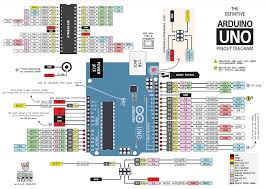
\includegraphics[width=0.8\linewidth]{../images/arduino_data}
\caption{Arduino Pinout Diagram}
\label{fig:arduino_data}
\end{figure}


\newpage

Me decido por Arduino UNO en base a los siguientes criterios:

\begin{itemize}
	\item{Precio reducido}, que oscila entre los 20 \euro
	\item{Potencia del procesador y menoría}, suficiente para soportar el firmware.
	\item{Conector USB tipo B}, al ser de buen tamaño, hace la conexión robusta.
	\item{Número de pines} suficiente para conectar todos los periféricos.
	\item{Características especiales}, (PWM y interrupciones hardware). 
	\item{I2C} compatible. 
\end{itemize}


\subsection{Módulo de motores}

Para permitir el control del motor de un paso a paso,  Pololu A4988 \cite{pololu},
las características más reseñables de tal controlador y que los hacen destacar frente a sus competidores.

\begin{itemize}
	\item{} Interfaz simple para controlar pasos y dirección.
	\item{} Cinco resoluciones de paso diferentes, paso completo, medio paso, cuarto de paso, octavo de paso, dieciseisava parte de paso. 
	\item{} Control de corriente de paso ajustable.
	\item{} Protecciones contra sobretensiones y sobrecalentamientos.
\end{itemize}


\begin{figure}[h]
\centering
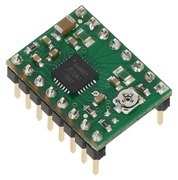
\includegraphics[width=0.3\linewidth]{../images/pololu}
\caption{Pololu A4988 Stepper Motor Driver Carrier}
\label{fig:pololu}
\end{figure}

\newpage

El motor empleado es un Motor paso a paso NEMA 17 / 3.2Kg/cm, de uso muy habitual, 
en el montaje de impresoras 3D,  

\bigskip
Sus características son las siguientes.

\begin{itemize}
	\item{Tamaño:} 42.3x48mm, sin incluir el eje (NEMA 17)
	\item{Peso:} 350 gramos (13 oz)
	\item{Diámetro del eje:} 5 mm "D"
	\item{Longitud del eje:} 25 mm
	\item{Pasos por vuelta:} 200 (1,8º/paso)
	\item{Corriente:}  1.2 Amperios por bobinado
	\item{Tensión:} 4 V
	\item{Resistencia:} 3.3 Ohm por bobina
	\item{Torque:} 3.2 kg/cm (44 oz-in)
	\item{Inductancia:} 2.8 mH por bobina 
\end{itemize}

\subsection{Módulo de pantalla}

Para visualizar los estados del sistema fácilmente, el sistema incorpora una pequeña pantalla LCD. 

Los más corrientes son los display LCD, de 16x2 o 16x4.

Para su utilización en un principio se estima controlarla mediante los pines digitales usando 4 señales digitales D7, D6, D5, y D4, junto con dos pines adicionales de control. Como podemos ver en los primeros diagramas.

En una fase de rediseño optimizamos el circuito incorporando una interfaz I2C \cite{I2C}, reduciendo las señales a solo dos. 


\subsection{Módulo sensores}

El dispositivo incorpora dos tipos de sensores:

\begin{itemize}
	\item Sensor térmico: Hacemos usos de  LM35 \cite{LM35},es un sensor de temperatura con una precisión calibrada de 1 \grad C. Su rango de medición abarca desde -55 \grad C hasta 150 \grad C. La salida es lineal y cada grado Celsius equivale a 10 mV.
	\item \textbf{Bumper sensor}, o contactos fines de carrera, son interruptores todo o nada, que se activan cuando se llega a límite físico. 
\end{itemize}


\subsection{Módulo control manual}

\begin{itemize}
	\item Potenciómetros, para regular algunos valores, en concreto usamos 10 kOhms.
	
	\item Botones, para unos primeros prototipos una botonera, para activar las funciones que me interesan.
	
	\item \textbf{Wii Nunchuck}, reutilizo un mando de la consola Wii, para de una forma ergonómica activar los comandos, mediante la zeta y algunos pulsadores, este mando es totalmente compatible dado que funciona bajo el protocolo I2C.
	 
\end{itemize}


\subsection{Módulo control remoto}

Para realizar el control remoto, hago uso de la comunicación serie que incorpora la placa Arduino.


El puerto serie envía la información mediante una secuencia de bits. Para ello se necesitan al menos dos conectores para realizar la comunicación de datos, RX (recepción) y TX (transmisión). 

En ocasiones veréis referirse a los puertos de serie como UART. La UART (universally asynchronous receiver/transmitter) es una unidad que incorporan ciertos procesadores, encargada de realiza la conversión de los datos a una secuencia de bits y transmitirlos o recibirlos a una velocidad determinada.

Los puertos serie están físicamente unidos a distintos pines, en Arduino UNO y Mini Pro los pines empleados son 0 (RX) y 1 (TX).


\begin{lstlisting}[language=C, caption={Ejemplo lectura y escritura puerto serie},label={lst:write_read_serial_port_sample}]

void setup(){
Serial.begin(9600);
}

void loop(){

}

void witeCharapter(char c){
	Serial.println(c);
}

void readCharapter(){
	if (Serial.available()>0){
		input=Serial.read();
		Serial.println(input);
}


\end{lstlisting}


Dado que tengo una cantidad de funciones a ejecutar mediante comandos, necesito formalizar un protocolo basado en mensajes preestablecidos. \\

Por seguir una nomenclatura, todos los comandos tienen el siguiente formato: \\


$ COMANDO?ARGUMENTO1?ARGUMENTO2  $

Y a continuación una lista de los comandos utilizados.


\begin{figure}[h]
\centering
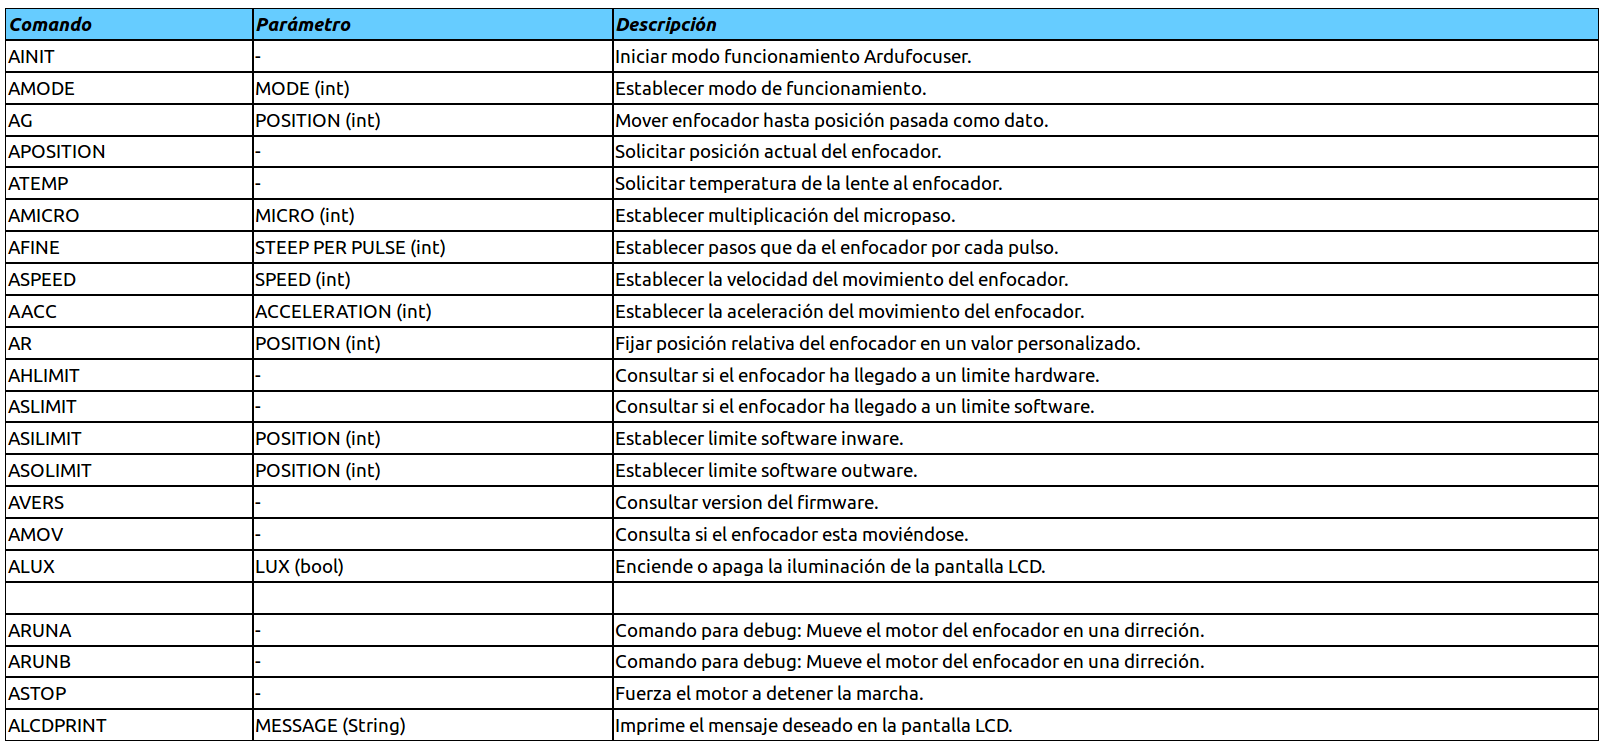
\includegraphics[width=1.1\linewidth]{../images/comando_ardufocuser}
\caption{}
\label{fig:comando_ardufocuser}
\end{figure}

Por regla general, todo comando tiene un mensaje de respuesta, bien indicando el nuevo estado del sistema que se ha cambiado (comandos escritura), bien información sobre el estado sobre el que solicitamos información (comandos lectura) o un ECHO del comando en algún otro caso.

\newpage


\section{Presupuesto}

\begin{itemize}
	\item Arduino UNO: 22\euro
	\item Motor PaP Nema 17: 10\euro
	\item Controladora Motor (Pololu o similar): 7\euro
	\item Pantalla LCD + controladora I2C: 2.5\euro
	\item Nunchaku Wii (compatible): 4\euro
	\item Sensor Temperatura, resistencias, condensador, led: 1\euro
	\item Cablecillos, soldadura, pines, placas, etc: 4\euro
	\item Potenciómetros: 2\euro
	\item Caja: 5\euro
	\item Clavijas aviador: 3\euro
	\item Fines de carrera: 2\euro
	
	
\end{itemize}
\textbf{Total: 62.5\euro}

\subsection{Integración de módulos}
\bigskip
Tras trabajar en cada uno de los módulos de forma independiente una visualización más o menos precisa es la siguiente:

\begin{figure}[h]
	\centering
	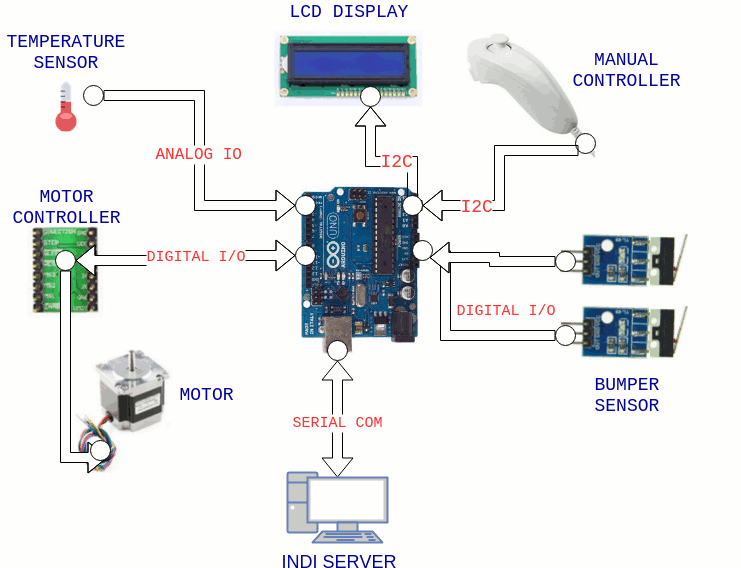
\includegraphics[width=0.9\linewidth]{../images/diagramaHardware}
	\caption{}
	\label{fig:diagramaHardware}
\end{figure}

Aún no tengo claro detalles como la alimentación de cada uno de los dispositivos,  exactamente las conexiones que va a requerir cada periférico ni su ubicación.

\bigskip
Es importante contabilizar número de pines que necesita cada periférico, si son digitales o analógico, pwd o hacen uso de interrupciones hardware. 

\bigskip
Con ello nos podemos hacer una idea aproximada del sistema y de los recursos que necesitamos.


\newpage
\section{Implementación hardware}

La implementación del dispositivo hardware, se puede definir como un proceso totalmente iterativo, en el marco del prototipado, comenzando por las pruebas de cada unos de los módulos, y trabajando con placas que permiten remover y cambiar la distribución de los componentes.



\begin{figure}[h]
\centering
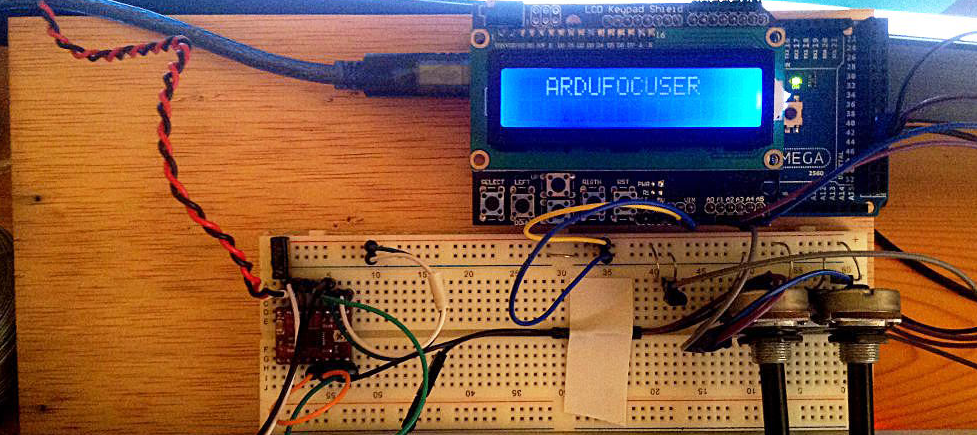
\includegraphics[width=0.7\linewidth]{../images/proto_recorte}
\caption{}
\label{fig:prototipoArdufocuser}
\end{figure}

\bigskip
Tras muchas pruebas y una vez claras las partes fundamentales de las que consta el dispositivo, así como su integración, se pasa a formalizar el diseño, buscando la elegancia, la máxima limpieza en la distribución de los componentes, así como la economía de espacio.

\begin{figure}[h]
	\centering
	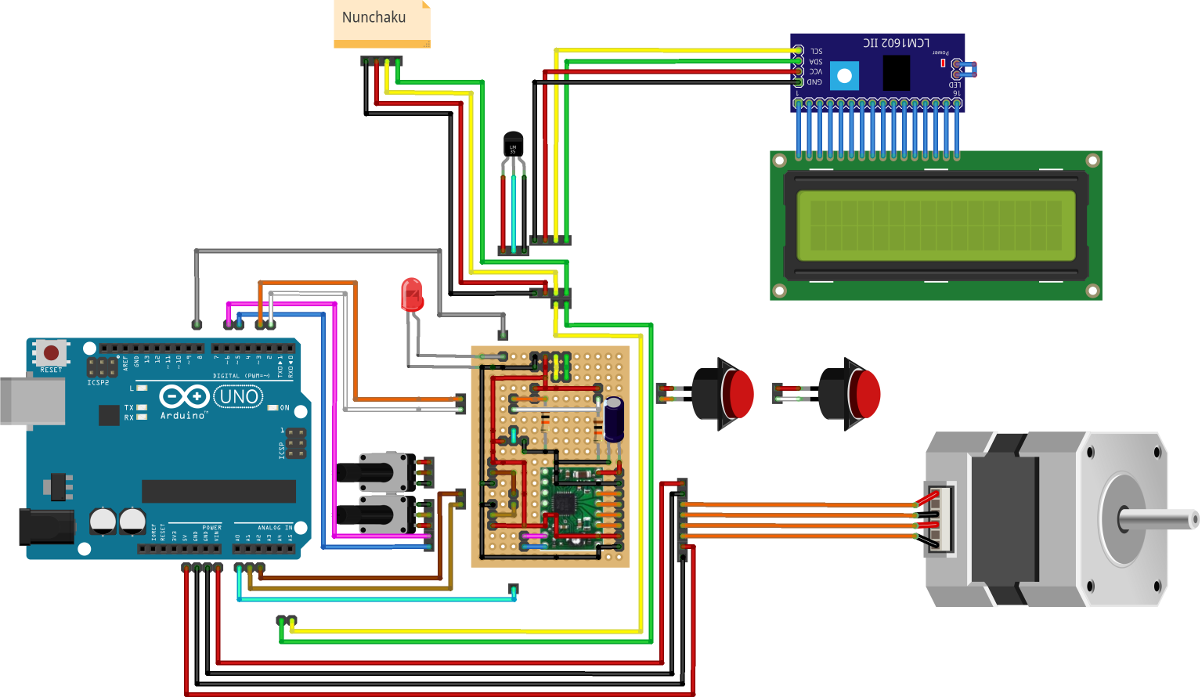
\includegraphics[width=1\linewidth]{../images/circuito}
	\caption{}
	\label{fig:prototipoArdufocuser}
\end{figure}


Una vez perfectamente definido el esquemático pasamos a la fase de soldadura.


\newpage

\section{Implementación firmware}


Con la experiencia y el trabajo, voy familiarizándome con la plataforma, conozco nuevas bibliotecas que me ayudan, nuevos periféricos,  así como mediante sesiones de refactorización, se consigue hacer código mantenible y modular. 

Es importante mencionar el uso de la herramienta \textbf{PlatformIO}, que se define a sí misma como un ecosistema abierto de desarrollo orientado a hardware. 


Tres son las características más sustanciales. 


- PlatformIO IDE: Un IDE orientado a la programación hardware, con funciones para facilitar la depuración, así como avisos para mejorar la calidad, totalmente configurado para compilar y cargar el programa directamente en una placa física, o en una placa virtual.

\begin{figure}
	\centering
	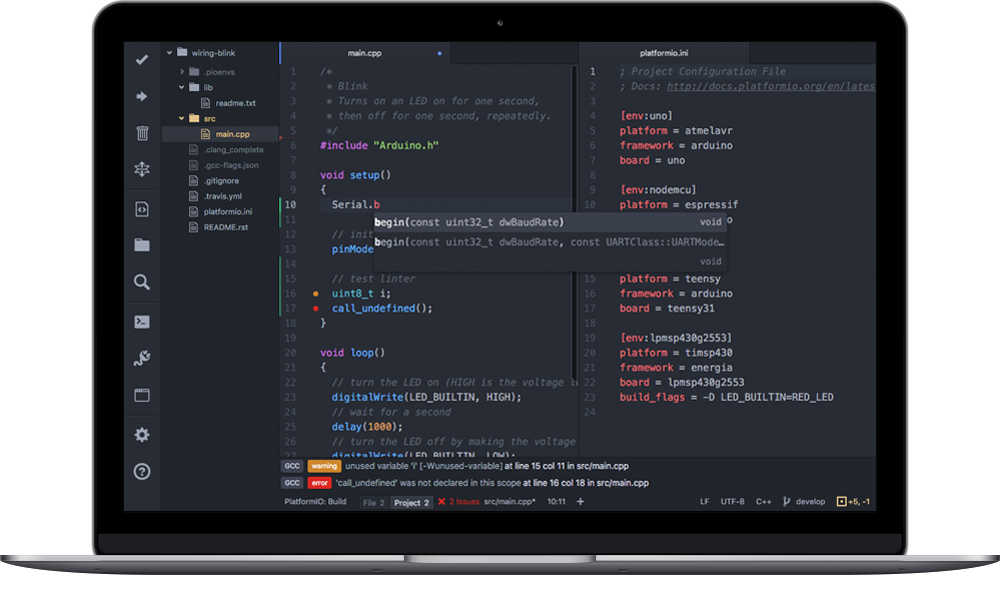
\includegraphics[width=0.7\linewidth]{../images/ide_arduino}
	\caption{}
	\label{fig:ide_arduino}
\end{figure}

- Terminal para realizar compilación en el cloud  para diferentes placas, así como permite compilación desde plataformas de integración continua como Travis CI.

- Gestor de bibliotecas y dependencias, tiene un repositorio con las bibliotecas más usadas, pudiendo buscar y actualizar rápidamente. 



El código fuente del firmware queda distribuido en los siguientes ficheros.

\begin{itemize}
	
\item $Ardufocuser-config.h$: Encapsula gran parte de la configuración, así como el mapeo de pines y demás definiciones. 
\item $Ardufocuser-init.h$: Inicializa el sistema, creando las instancias de los objetos utilizados, variables globales, contadores y demás estados.
\item $Ardufocuser-cmd.h$: Se definen los comandos remotos, junto con sus funciones callback asociadas.
\item $Ardufocuser-utils.h$: Incorpora algunas funciones de propósito general útiles en algunos de los módulos. 
\item $Ardufocuser.ino$: Es el script principal, incluye los ficheros anteriores, contiene las funciones setup(),  loop() y callback de las interrupciones hardware y software.

\item $library.json$: Hace referencia a las librerías de terceros, catalogadas, y con referencias al sitio web y al desarrollador o equipo de desarrollo. Por seguridad también las incorporo al repositorio en el directorio libs.  


\end{itemize}
\newpage
\begin{lstlisting}[language=C, caption={Núcleo implementación firmware  ardufocuser},label={lst:nucleo_firmware_ardufocuser }]

	void setup()
	{
		//Inicia comunicación serie.
		Serial.begin(9600);
		
		// Inicia pantalla LCD.
		lcd.begin();
		lcd.backlight();
		
		// Saludo inicial.
		welcome("   ARDUFOCUSER  ");
		
		// Velocidad y Aceletación inicial del motor.
		motor.setMaxSpeed(200);
		motor.setAcceleration(1000);
		
		//Iniciamos control Nunckuck
		chuck.begin();
		chuck.update();
		
		// Actualizamos con datos guardados en sesion anterior
		load_session();
		
		// Iniciamos interrupciones Software.
		// Gestiona movimiento del motor.
		Timer1.initialize(50);
		Timer1.attachInterrupt(timerFunction);
		
		// Inicia interrupciones hardware a la escucha.
		attachInterrupt ( 0, finA,RISING);
		attachInterrupt ( 1, finB,RISING);
		
		// Registramos y iniciamos comandos serie.
		registerCommand();
	}
	
	void loop()
	{
		// Leemos nuevo comando serie.
		serial_cmd.readSerial();
		
		// Leemos control manual y sensores auxiliares.
		read_manual_controller();
		
		// Actualizamos LCD.
		update_lcd_display();
		
		// Leemos controles nunchuck.
		nunckuck_controller();
		
		// Almacenamos estados de forma persistente 
		// para otra sesión.
		save_current_session();
	}



\end{lstlisting}



\section{Pruebas sobre el dispositivo hardware.}


La sección de pruebas las dividimos en varias partes, pruebas de concepto de cada uno de los componentes y módulos individuales, pruebas de integración, pruebas de rendimiento. 

Además para asegurar que el firmware implementado, permite ser compilado en las distintas placas hacemos uso del framework   \textbf{PlatformIO} \cite{patform}.





- Buscador centralizado de bibliotecas, en los proyectos Arduino es uno de los problemas, dado que cada una de ellas puede provenir de una fuente totalmente diferente, con esta herramienta contamos con un solo lugar.

 
 
\newpage
\begin{lstlisting}[language=python, caption={Script travis para realizar integración continua},label={lst:write_read_serial_port_sample}]

language: python
python:
- "2.7"

install:
- python -c "$(curl -fsSL https://raw.githubusercontent.com/platformio/platformio/master/scripts/get-platformio.py)"
- wget https://github.com/josemlp91/ardufocuser_firmware/raw/master/Ardufocuser/libs/TimerOne.zip
- unzip TimerOne.zip
- wget https://github.com/josemlp91/ardufocuser_firmware/raw/master/Ardufocuser/libs/i2clcd.zip
- unzip i2clcd.zip
- wget https://github.com/josemlp91/ardufocuser_firmware/raw/master/Ardufocuser/libs/AccelStepper-1.49.zip
- unzip AccelStepper-1.49.zip
- wget https://github.com/josemlp91/ardufocuser_firmware/raw/master/Ardufocuser/libs/nunchuck.zip
- unzip nunchuck.zip


script:
- platformio ci Ardufocuser --lib="TimerOne" --lib="i2clcd" --lib="nunchuck" --lib="AccelStepper" --board=uno

\end{lstlisting}


\begin{figure}[h]
\centering
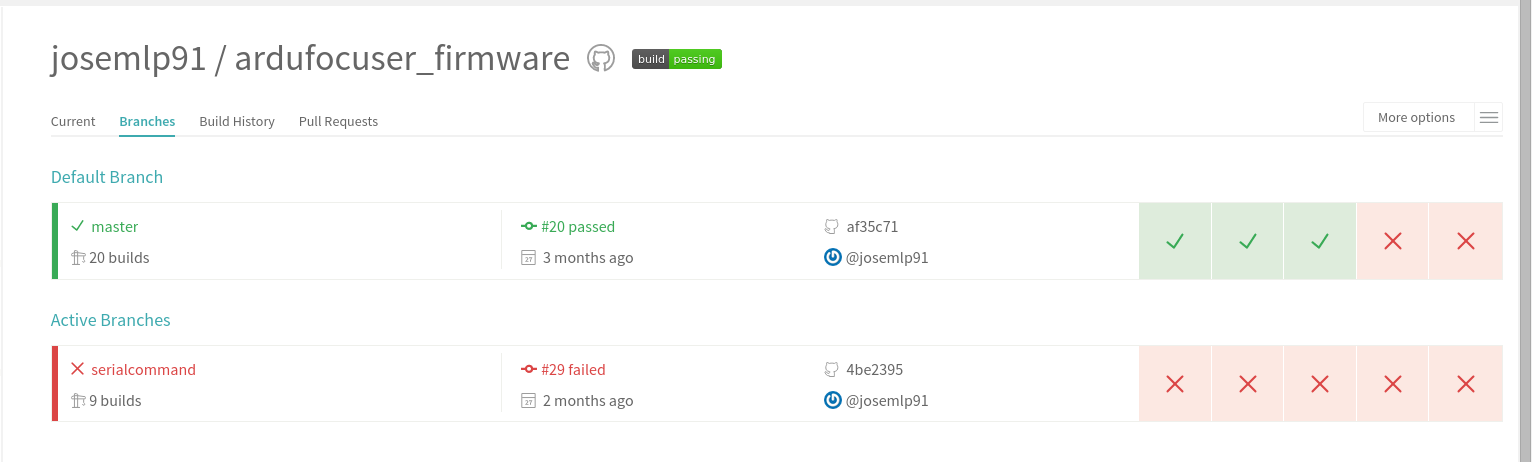
\includegraphics[width=1\linewidth]{../images/travis_ci}
\caption{}
\label{fig:travis_ci}
\end{figure}




\begin{figure}[h]
	\centering
	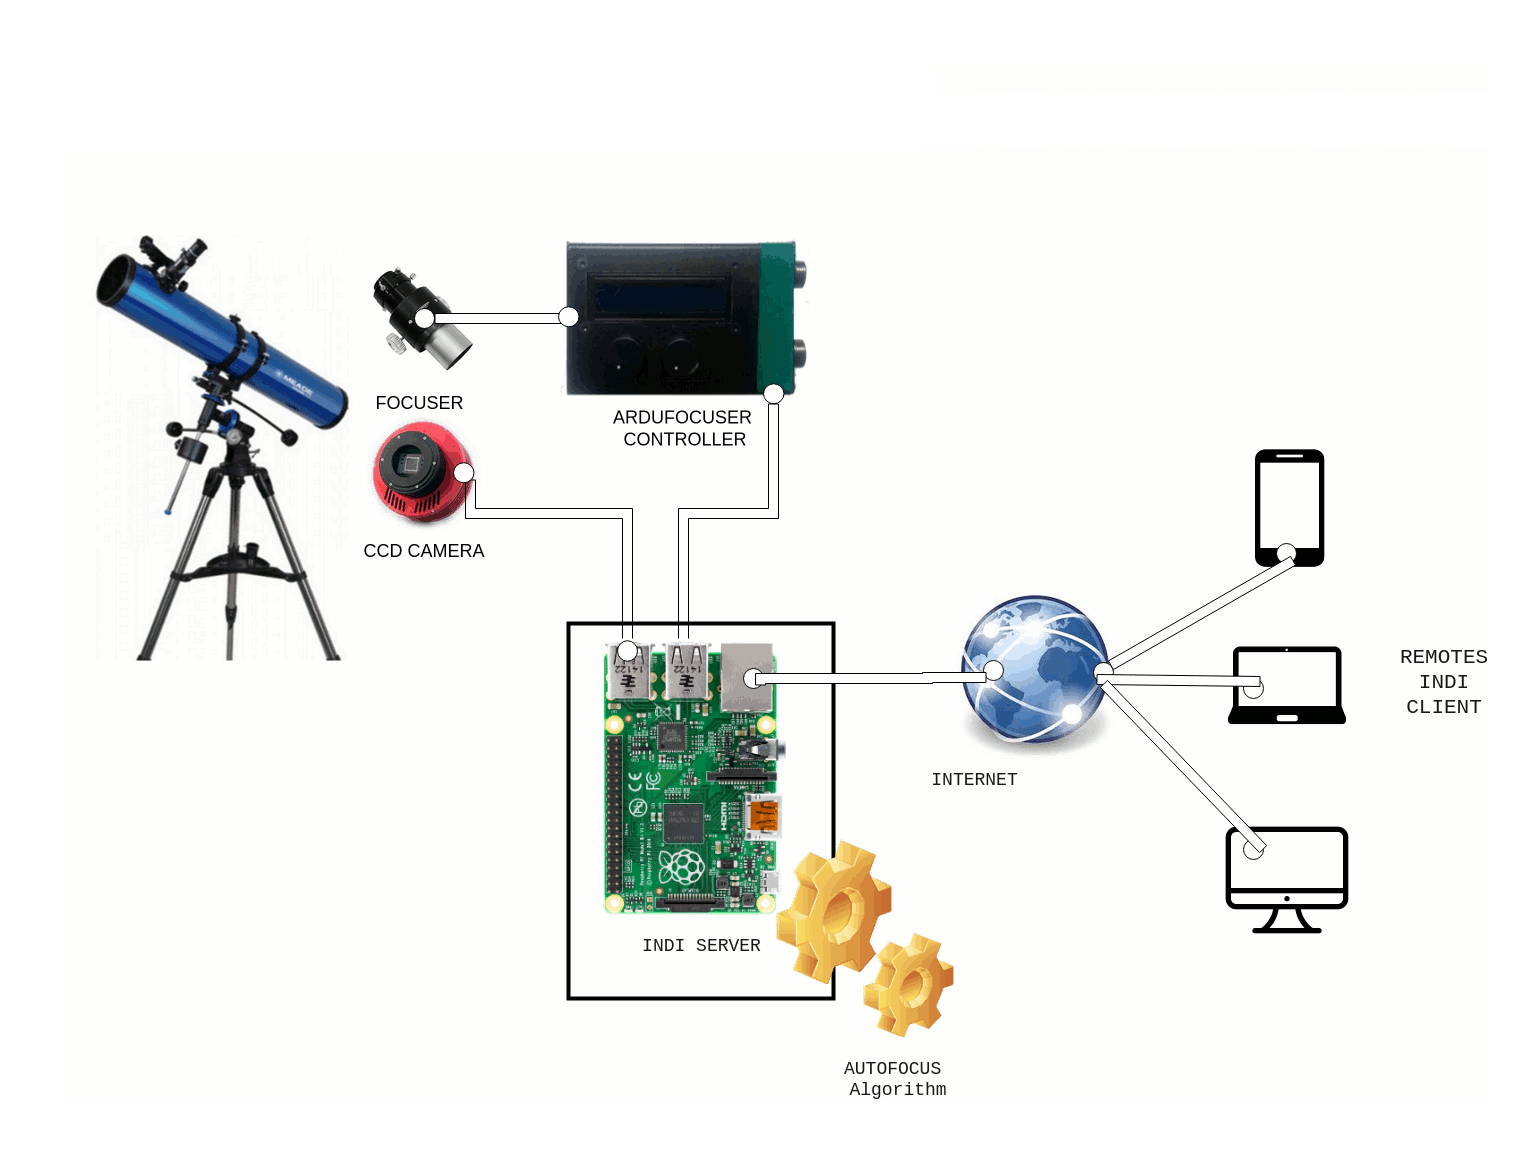
\includegraphics[width=0.7\linewidth]{../images/diagramaGeneral}
	\caption{}
	\label{fig:diagramaHardware}
\end{figure}


\begin{figure}[h]
	\centering
	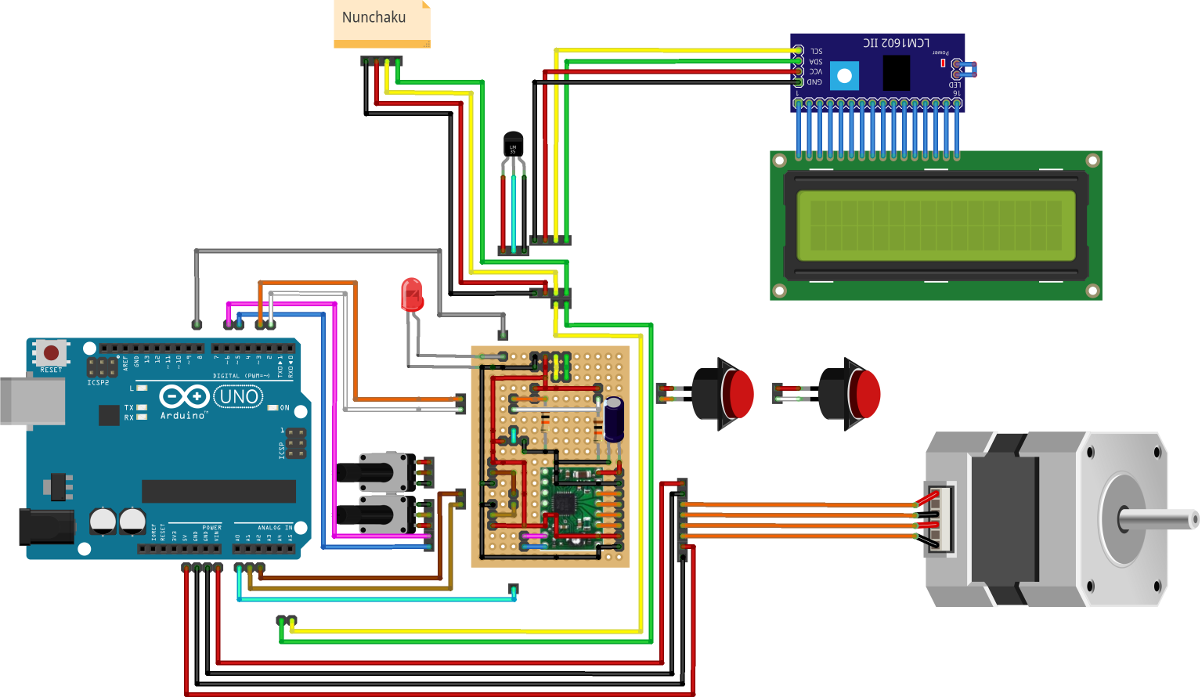
\includegraphics[width=0.7\linewidth]{../images/circuito}
	\caption{}
	\label{fig:diagramaHardware}
\end{figure}


